%%%%%%%%%%%%%%%%%%%%%%%%%%%%%%%%%%%%%%%%%%%%%%%%%%%
%% P3: Phenomenology of Particle Physics                         
%%
%% Author:  André Rubbia                   		 
%%
%% Figure 11.2 Angular dependence of the Mott scattering cross-section compared to the Rutherford formula.
%%
%% This work is licensed under the Creative Commons Attribution 4.0 International License. 
%% To view a copy of this license, visit http://creativecommons.org/licenses/by/4.0/ or 
%% send a letter to Creative Commons, PO Box 1866, Mountain View, CA 94042, USA.
%%
%%%%%%%%%%%%%%%%%%%%%%%%%%%%%%%%%%%%%%%%%%%%%%%%%%%

\documentclass[a4paper,10pt]{article}

\usepackage[T1]{fontenc}
\usepackage[utf8]{inputenc}
\usepackage{lmodern}
\usepackage[labelfont=bf]{caption}
\usepackage{upgreek}

\usepackage{tikz}
\usepackage{pgfplots}
\pgfplotsset{compat=1.17}
\usepgfplotslibrary{ternary}
\usepgfplotslibrary{fillbetween}
\usepgfplotslibrary{external}

\usepackage{braket}

\def\d{\mathrm{d}}

\begin{document}

%%%%%%%%%%%%%%%%% FIGURE %%%%%%%%%%%%%%%%%%%%%%%%%%%%%%%%%%
\begin{figure}[htb]
\begin{center}
\pgfplotsset{every axis/.append
    style={
    line width=1pt,
    tick style={line width=0.8pt}}}
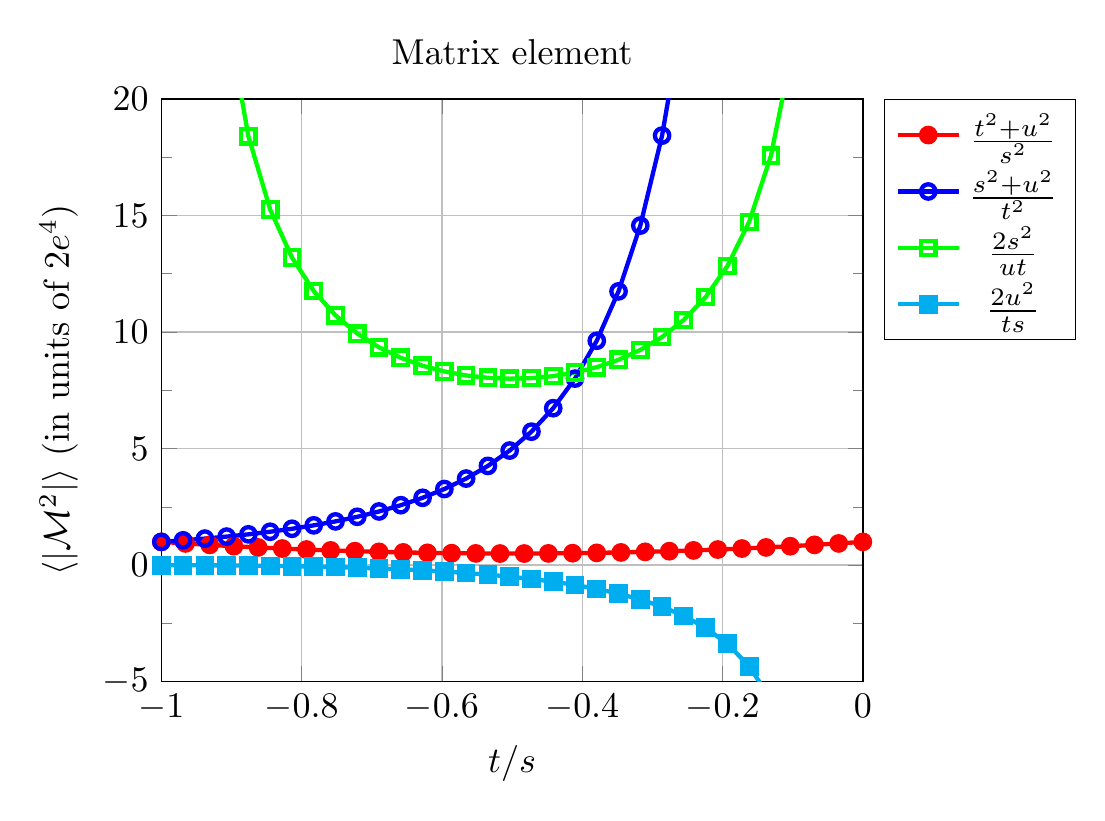
\begin{tikzpicture}[scale=1.3]
    \begin{axis}[
        title=Matrix element,
        xlabel={$t/s$},
        ylabel={$\braket{\vert{\cal M}^2\vert}$ (in units of $2e^4$)},
        xmin=-1, xmax=0,
        ymin = -5, ymax=20,
        minor y tick num=1,
        grid = major,
        legend entries={
        $\frac{t^2+u^2}{s^2}$,
        $\frac{s^2+u^2}{t^2}$,
        $\frac{2s^2}{ut}$,
        $\frac{2u^2}{ts}$
        },
        legend style={legend pos = outer north east}
    ]
       \addplot [red,very thick, samples=30,domain=-1:0, mark=*] {x^2+(1+x)^2};
        \addplot [blue,very thick,samples=30,domain=-1:-0.1,mark=o] {(1/x)^2+((1+x)/x)^2};
        \addplot [green,very thick, samples=30,domain=-1:-0.1,mark=square] {-2/(x*(1+x))};
        \addplot [cyan,very thick, samples=30,domain=-1:-0.1, mark=square*] {(1+x)/x*(1+x)};
   \end{axis}
\end{tikzpicture}%
\caption{Graphical plot of the different terms
in the matrix elements as a function of $t/s$. The $u$  variable is given by
$u/s=-(1+t/s)$. The interference terms are also shown separately.}
\label{fig:qedmainprocessesmandeldep}
\end{center}
\end{figure}
%%%%%%%%%%%%%%%%% END FIGURE %%%%%%%%%%%%%%%%%%%%%%%%%%%%%%
%

\end{document}
